\acs{GNU} Radio is a development toolkit to build your own software radio or signal processing application. The applications can be combined with external radio-frequency hardware or simulated.
\newline
Due to the broad field of application \acs{GNU} Radio is used by a lot of hobby radio operators, academic facilities and commercial environments \cite{gnu_radio_website_welcome_????}.
\newline
To build these applications, a graphical tool, \ac{GRC}, is provided to draw a signal flowgraph.
\begin{figure}[ht!]
\centering
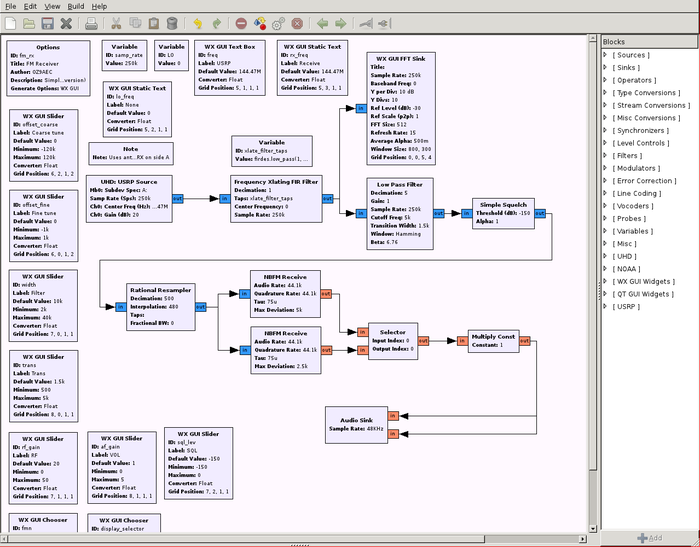
\includegraphics[width=120mm]{PICs/GRC_flowgraph.jpg}
\caption[Editing a flowgraph in \acl{GRC} - licensed under the \acl{GNU GPL} \cite{gnu_radio_website_grc_????}]{Editing a flowgraph in \acl{GRC} - licensed under the \acl{GNU GPL} \label{GRCFlowgraph}}
\end{figure}
\newline
One of the applications based on the \acs{GNU} Radio is \ac{FLdigi}. This or an adapted version like Dl-\ac{FLdigi} could be used to convert the data the \acp{GCC} receive from the \ac{MCC} to the protocol the satellite uses.